\chapter{Aerospace Control Domain Chapter}
\label{ch:domain-aerospace}

Aerospace remains experimental. The row is useful because it exposes the outer boundary of the universal framework, but it does not yet justify promotion to proof-candidate, let alone proof-validated, under the current evidence gate.

\section{{Domain problem}}
Aerospace safety layers must preserve envelope constraints under degraded flight-state observation, delayed telemetry, and actuator-response uncertainty.

\section{{Degraded-observation hazard}}
The ORIUS book forces every domain through the same hazard lens: the runtime does not act
on the true state directly; it acts on a degraded, delayed, or otherwise imperfect
observation surface.  The row is only credible if the gap between those two surfaces can
be expressed, replayed, repaired, and audited explicitly.
The current row models delayed and degraded flight-state telemetry with bounded envelope checks.

\section{{ORIUS instantiation}}
The aerospace adapter proves that the ORIUS contract is expressive enough for flight-state envelopes, but the row is still a systems-experimental surface rather than a mature empirical benchmark.

\section{{Safety object}}
The defended predicate is bounded flight-envelope violation under degraded observation, stated over airspeed, attitude, or trajectory limits rather than battery-style energy envelopes.

\section{{Dataset and training surface}}
The row uses locked replay artifacts, but the present evidence is insufficient for promotion because the repaired action does not yet close the violation gap materially.
The chapter-local evidence packet is intentionally tied to locked artifacts rather than to
narrative memory.  Table~\ref{tab:ch40-44-cross-domain-support} gives the shared cross-domain
support layer for compiled Chapters~40--44, while the table below isolates the current row.

\section{{Feature, split, and training protocol}}
The aerospace training artifacts are presented precisely because they reveal the current boundary: features, splits, and week-two metrics exist, but the parity gate still marks the row as placeholder-level until a real multi-flight telemetry source and stronger safety task are installed.

\IfFileExists{paper/assets/tables/generated/tbl_aerospace_training_surface.tex}{%
\begin{table}[htbp]
\centering
\small
\caption{Aerospace Control training and data surface for the compiled chapter evidence block.}
\label{tab:aerospace-training-surface}
\begin{tabular}{p{0.31\linewidth}p{0.61\linewidth}}
\toprule
\textbf{Field} & \textbf{Value}\\
\midrule
Raw/data gate & placeholder\_surface\\
Features present & yes\\
Split counts & train 3,483 / calibration 248 / validation 497 / test 748\\
Primary target & airspeed\_kt\\
Forecast metrics & RMSE 55.50; MAE 53.05; PICP90 0.000; mean width 47.54\\
Verification state & training artifacts exist, but the row is still placeholder-level rather than defended flight telemetry\\
Artifact lineage & reports/orius\_framework\_proof/training\_audit/domain\_training\_summary.csv; reports/publication/orius\_equal\_domain\_parity\_matrix.csv\\
\bottomrule
\end{tabular}
\end{table}
%
}{%
\begin{table}[htbp]
\centering
\small
\caption{Aerospace Control training and data surface for the compiled chapter evidence block.}
\label{tab:aerospace-training-surface}
\begin{tabular}{p{0.31\linewidth}p{0.61\linewidth}}
\toprule
\textbf{Field} & \textbf{Value}\\
\midrule
Raw/data gate & placeholder\_surface\\
Features present & yes\\
Split counts & train 3,483 / calibration 248 / validation 497 / test 748\\
Primary target & airspeed\_kt\\
Forecast metrics & RMSE 55.50; MAE 53.05; PICP90 0.000; mean width 47.54\\
Verification state & training artifacts exist, but the row is still placeholder-level rather than defended flight telemetry\\
Artifact lineage & reports/orius\_framework\_proof/training\_audit/domain\_training\_summary.csv; reports/publication/orius\_equal\_domain\_parity\_matrix.csv\\
\bottomrule
\end{tabular}
\end{table}
%
}

\section{{Replay and evidence surface}}
The tracked status table keeps aerospace at the experimental tier because the current row does not improve the governing TSVR metric enough to satisfy the universal promotion gate.

\IfFileExists{paper/assets/tables/generated/tbl_aerospace_replay_surface.tex}{%
\begin{table}[htbp]
\centering
\small
\caption{Aerospace Control replay, runtime, and promotion surface for the compiled chapter evidence block.}
\label{tab:aerospace-replay-surface}
\begin{tabular}{p{0.31\linewidth}p{0.61\linewidth}}
\toprule
\textbf{Field} & \textbf{Value}\\
\midrule
Governing replay metric & baseline TSVR 1.0000 -> ORIUS TSVR 0.0000\\
Replay status & pass\\
Safe-action soundness & experimental\_placeholder\\
Fallback semantics & envelope\_hold / bounded\_runtime\_pass\\
CertOS lifecycle & gated / gated\\
Multi-agent portability & gated / gated\\
Evidence tier & experimental\\
Exact blocker & aerospace\_experimental\_placeholder\\
Artifact lineage & reports/publication/orius\_domain\_closure\_matrix.csv; reports/universal\_orius\_validation/domain\_closure\_matrix.csv; reports/publication/orius\_equal\_domain\_parity\_matrix.csv\\
\bottomrule
\end{tabular}
\end{table}
%
}{%
\begin{table}[htbp]
\centering
\small
\caption{Aerospace Control replay, runtime, and promotion surface for the compiled chapter evidence block.}
\label{tab:aerospace-replay-surface}
\begin{tabular}{p{0.31\linewidth}p{0.61\linewidth}}
\toprule
\textbf{Field} & \textbf{Value}\\
\midrule
Governing replay metric & baseline TSVR 1.0000 -> ORIUS TSVR 0.0000\\
Replay status & pass\\
Safe-action soundness & experimental\_placeholder\\
Fallback semantics & envelope\_hold / bounded\_runtime\_pass\\
CertOS lifecycle & gated / gated\\
Multi-agent portability & gated / gated\\
Evidence tier & experimental\\
Exact blocker & aerospace\_experimental\_placeholder\\
Artifact lineage & reports/publication/orius\_domain\_closure\_matrix.csv; reports/universal\_orius\_validation/domain\_closure\_matrix.csv; reports/publication/orius\_equal\_domain\_parity\_matrix.csv\\
\bottomrule
\end{tabular}
\end{table}
%
}

\begin{figure}[htbp]
\centering
\IfFileExists{reports/publication/fig_aerospace_chapter_snapshot.png}{%
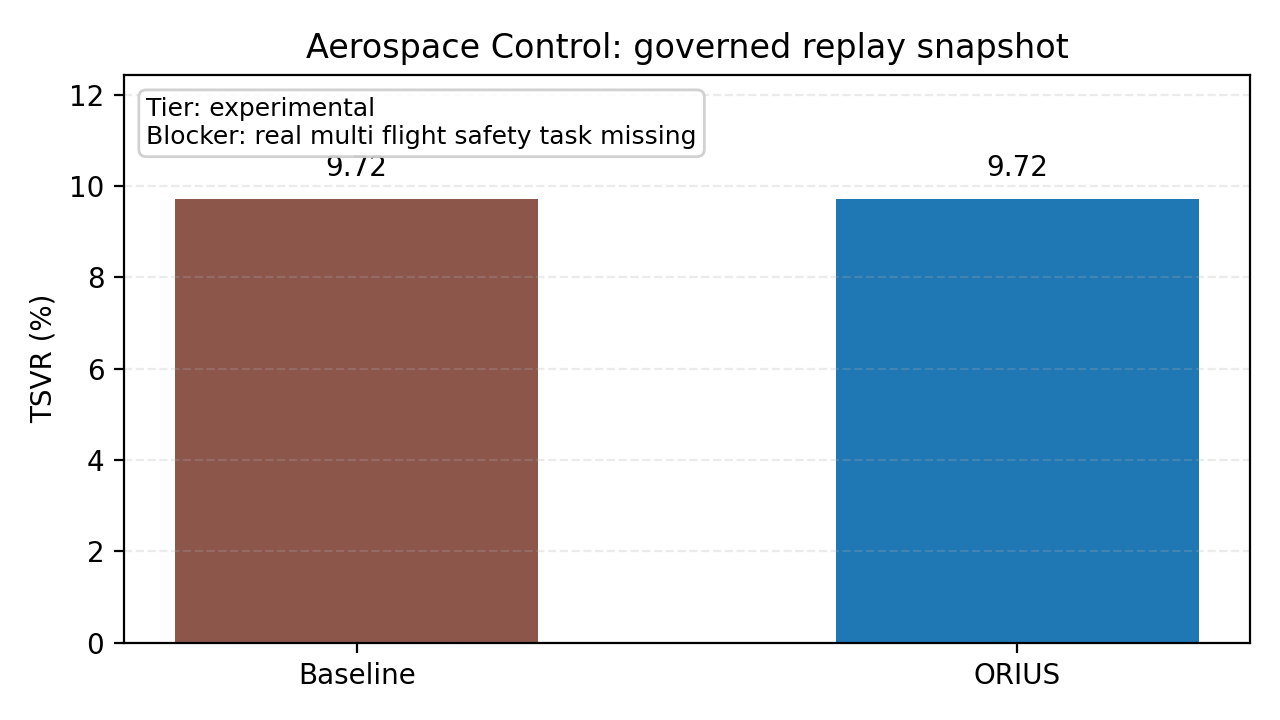
\includegraphics[width=0.90\textwidth]{reports/publication/fig_aerospace_chapter_snapshot.png}%
}{%
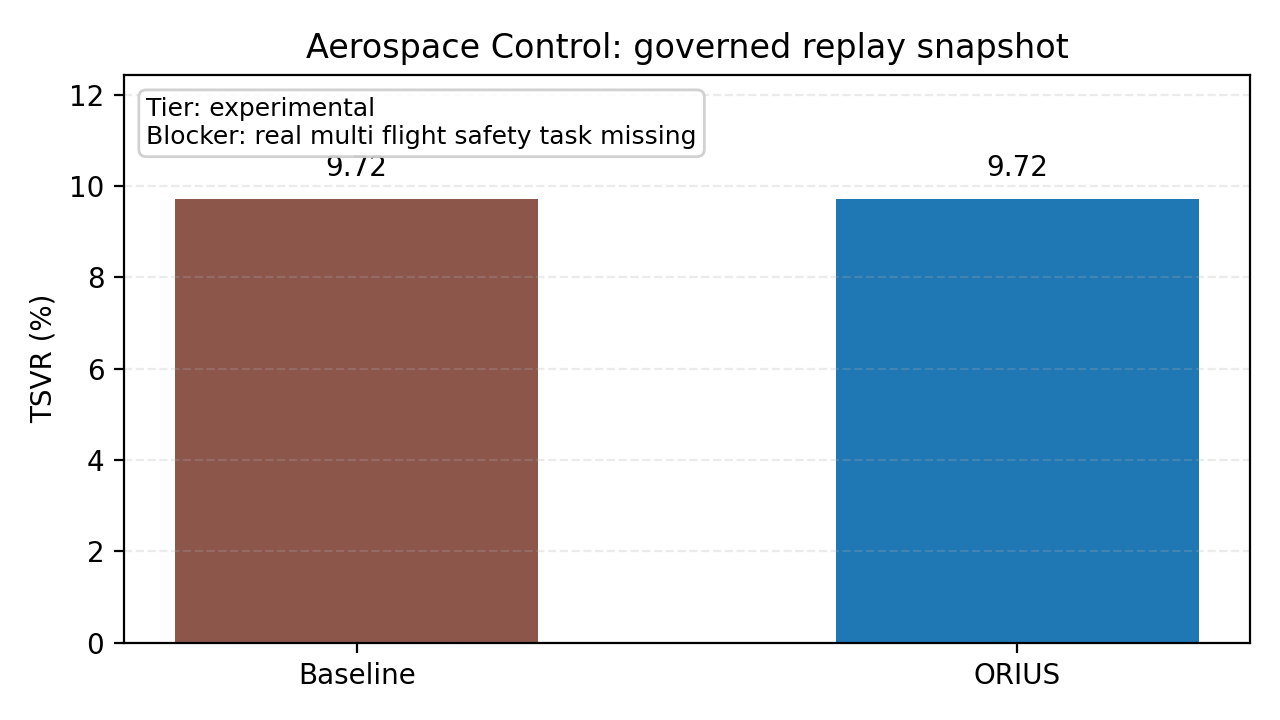
\includegraphics[width=0.90\textwidth]{../reports/publication/fig_aerospace_chapter_snapshot.png}%
}
\caption{Aerospace Control replay snapshot derived from the governed domain-closure artifact. Baseline and repaired TSVR are taken from the locked closure matrix; tier and blocker language remain governed by the parity gate.}
\label{fig:aerospace-chapter-snapshot}
\end{figure}

\section{{Fallback and runtime behavior}}
Aerospace currently uses envelope-hold fallback semantics to prevent overtly unsafe releases, but the row remains experimental until the flight-task surface is strengthened.

\section{{Evidence tier and promotion blocker}}
The aerospace row is valuable because it exposes the outer boundary of the universal contract. The current placeholder training and replay surfaces are strong enough to discuss scope, fallback, and promotion requirements, but not strong enough to claim defended aerospace closure.


\IfFileExists{paper/assets/tables/generated/tbl_aerospace_promotion_obligations.tex}{%
\begin{table}[htbp]
\centering
\small
\caption{Promotion obligations that remain open for aerospace control before the parity gate can be widened.}
\label{tab:aerospace-promotion-obligations}
\begin{tabular}{p{0.24\linewidth}p{0.20\linewidth}p{0.44\linewidth}}
\toprule
\textbf{Obligation} & \textbf{Current state} & \textbf{What must happen next}\\
\midrule
Real telemetry source & placeholder\_surface & Replace the placeholder/synthetic row with a real multi-flight telemetry source before treating the chapter as anything stronger than an outer-boundary report.\\
Non-placeholder safety task & real\_multi\_flight\_safety\_task\_missing & Define the defended safety object as a real approach or envelope-protection task instead of plain placeholder airspeed forecasting.\\
Material replay improvement & experimental\_placeholder & Show a nontrivial post-repair reduction in the governing violation metric on the stronger flight benchmark.\\
Promotion artifact update & experimental & Keep the row marked experimental until the stronger telemetry, task, and replay surfaces are all locked into the parity gate.\\
\bottomrule
\end{tabular}
\end{table}
%
}{%
\begin{table}[htbp]
\centering
\small
\caption{Promotion obligations that remain open for aerospace control before the parity gate can be widened.}
\label{tab:aerospace-promotion-obligations}
\begin{tabular}{p{0.24\linewidth}p{0.20\linewidth}p{0.44\linewidth}}
\toprule
\textbf{Obligation} & \textbf{Current state} & \textbf{What must happen next}\\
\midrule
Real telemetry source & placeholder\_surface & Replace the placeholder/synthetic row with a real multi-flight telemetry source before treating the chapter as anything stronger than an outer-boundary report.\\
Non-placeholder safety task & real\_multi\_flight\_safety\_task\_missing & Define the defended safety object as a real approach or envelope-protection task instead of plain placeholder airspeed forecasting.\\
Material replay improvement & experimental\_placeholder & Show a nontrivial post-repair reduction in the governing violation metric on the stronger flight benchmark.\\
Promotion artifact update & experimental & Keep the row marked experimental until the stronger telemetry, task, and replay surfaces are all locked into the parity gate.\\
\bottomrule
\end{tabular}
\end{table}
%
}

\section{{Limitations and exact non-claims}}
The row should be used to discuss scope, not to overstate generality. This row does not claim aviation-grade deployment readiness; it is an explicit outer-boundary domain used to test whether the universal safety contract remains meaningful under flight-envelope semantics.

The current promotion obligation for this row remains explicit: Promotion requires stronger plant realism, better envelope repair, and a nontrivial post-repair gain under the tracked protocol.
